\section{Эксперемент}
\subsection{Часть}
\begin{eqnarray}
    H_2O + e^- &\to&  HO^- + H \\
    Cl^- - e^- &\to& Cl  
\end{eqnarray}


\begin{equation}
    2NaCl + 2H_2O \to H_2\uparrow + 2NaOH + Cl_2\uparrow
\end{equation}

Катод окрашивается из-за фенол фталеина в щелочной среде $\inner{KOH}$, 
на катоде выделятся $Cl_2$ кислотный газ и индикаторная бумага темнеет.

\begin{figure}[h]
    \centering
    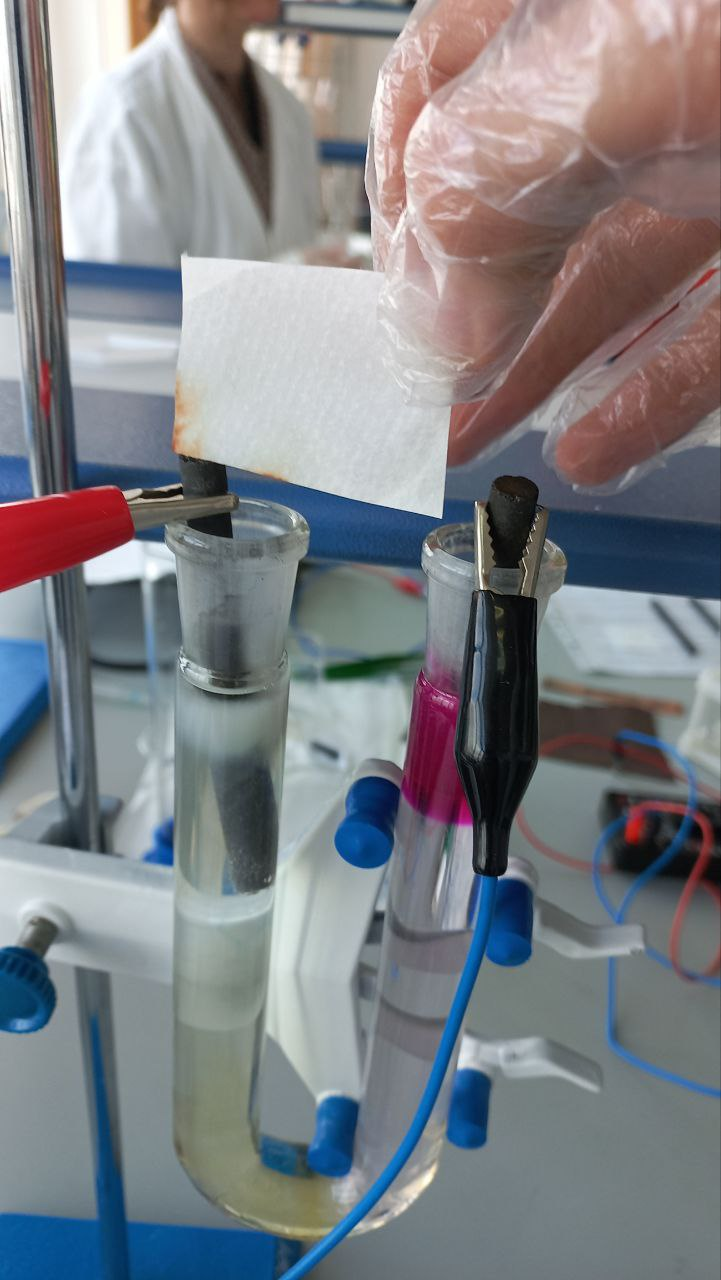
\includegraphics[trim={0 15cm 0 10cm},clip,width=\textwidth]{Ex_5/Ex_5_2.jpg}
     \caption{Результыты эксперемента}
    \label{Ex_5_2}
\end{figure}

\subsection{Часть}
\begin{eqnarray}
    H_2O + e^- &\to&  HO^- + H \\
    I^- - e^- &\to& I  
\end{eqnarray}


\begin{equation}
    2KI + 2H_2O \to H_2\uparrow + 2KOH + I_2\uparrow
\end{equation}

Катод окрашиватся из-за фенол фталеина в щелочной среде,  
на аноде выделятся $I_2$ реагирует с крахмалом и дает очень 
сильно насыщенный синий цвет.

\subsection{Часть}
\begin{eqnarray}
    H_2O + e^- &\to&  HO^- + H | \cdot 2 \\
    2Cl^- - 2e^- &\to& Cl
\end{eqnarray}

\begin{equation}
    ZnCl_2 + H_2O \to H_2\uparrow + KOH + Cl_2\uparrow
\end{equation}

\subsection{Часть}

\begin{eqnarray}
    H_2O + e^- &\to&  HO^- + H \\
    Cl^- - e^- &\to& Cl  
\end{eqnarray}




